\documentclass{article}

\usepackage[utf8]{inputenc}
\usepackage[T1]{fontenc}
\usepackage[greek,english]{babel}
\usepackage{alphabeta}
\usepackage{amsmath}
\usepackage{amssymb}
\usepackage{graphicx}
\usepackage{subcaption}
\usepackage{epstopdf}
\usepackage[margin=1in, paperwidth=7.5in,paperheight=10.5in]{geometry}
\usepackage{hyperref}
\usepackage{paracol}

\newcommand\course{ΗΡΥ 411}
\newcommand\courseName{Ενσωματωμένα Συστήματα Μικροεπεξεργατών}
\newcommand\semester{Χειμερινό 2020-2021}
\newcommand\assignmentNumber{Εργαστήριο 2}
\newcommand\studentName{Μαυρογιώργης Δημήτρης}                           
\newcommand\studentNumber{2016030016}

\title{\underline{\textbf{\assignmentNumber}}} 
\author{\textsc{\textbf{Όνομα:}}  \studentName\\
		\textsc{\textbf{ΑΜ:}}  \studentNumber\\
		\course \ - \courseName\\ 
		\textsc{Πολυτεχνείο Κρήτης}
		}
\date{\today}
\begin{document}
	\maketitle

\section*{Σκοπός}
	Σκοπός του δεύτερου εργαστηρίου είναι η περαιτέρω εξοικείωση μας με το περιβάλλον ανάπτυξης μικροελεγκτών AVR. Ειδικότερα, στόχος του εργαστηρίου είναι η δημιουργία ενός προγράμματος για οδήγηση με πολυπλεξία στον χρόνο μίας οθόνης 7-segment LED οκτώ ψηφίων. Για την πολυπλεξία το χρόνο, χρησιμοποιήθηκε ο timer/counter0 και τα interrupt από το πρώτο εργαστήριο, προκειμένου να διαιρέσουμε το χρόνο σε slots και σε κάθε slot να έχουμε ενεργό ένα LED στο οποίο εμφανίζουμε έναν αριθμό BCD.

\section*{Περιγραφή της υλοποίησης}
	Για το συγκεκριμένο εργαστήριο χρησιμοποιήθηκαν η θύρα Α του AVR για το περιεχόμενο του κάθε 7-segment και η θύρα C για την ενεργοποίηση του κάθε ψηφίου που βγαίνει στην οθόνη. Επιπλέον, τόσο τα δεδομένα προς εμφάνιση, όσο και τα δεδομένα για το ποιο LED ανάβουμε βρίσκονται στην κυρίως μνήμη. Πιο συγκεκριμένα, για τα περιεχόμενα των 7-segment χρησιμοποιήθηκε η διεύθυνση 0x60 έτσι, ώστε κάθε φορά που διαβάζουμε έναν BCD αριθμό προς εμφάνιση να προσθέτουμε στη διεύθυνση αυτή τον αριθμο και να παίρνουμε τη διεύθυνση στην οποία υπάρχει η αποκωδικοποίηση του αριθμού για τα 7-segments. Επίσης, για τα δεδομένα προς εμφάνιση χρησιμοποιήθηκε η διεύθυνση 0x76.\\
	
	\noindent
	Παράλληλα, επειδή ήταν αναγκαία η χρήση ενός timer, για την ανανέωση των LED, χρησιμοποιήθηκε ο κώδικας του δεύτερου μερους του πρώτου εργαστηρίου με τον timer/counter0 και τα interrupts. Πιο ειδικά, για το κάθε LED θέλαμε μια ελάχιστη συχνότητα 30 Hz. Eπομένως, το 1 ms του πρώτου εργαστηρίου ήταν επαρκές για την ανανέωση του κάθε ψηφίου. \\

	\noindent
	\textbf{Επεξήγηση Κώδικα} \\
	\noindent
	Aρχικά, στο data segment πρέπει να κάνουμε memory allocation για τις δέκα αποκωδικοποιήσεις των BCD αριθμών, καθώς και για τους οχτώ αριθμούς που θέλουμε να εμφανίσουμε. Επιπρόσθετα, αρχικοποιούμε τους καταχωρητές DDRA και DDRC με 0xFF, επειδή η θύρα A και C είναι έξοδοι, καθώς και τους PORTA και PORTC με 0xFF και 0x00 αντίστοιχα.\\
	
	\noindent
	Επίσης, οι αρχικοποιήσεις των καταχωρητών TCNT, TCCR0 και TIMSK είναι οι ίδιες με του εργαστηρίου 1, καθώς θἐλουμε κάθε 1 ms να ανανεώνονται τα LED. Αφού έγινε η αποθήκευση των 18 τιμών στη μνήμη, αρχικοποιούμε τους καταχωρητές Χ και Υ με τις διευθύνσεις 0x60 και 0x76 που αποθηκεύσαμε τα δεδομένα. Οι συγκεκριμένοι καταχωρητές θα χρησιμεύσουν για να διαβάζουμε κάθε φορά από τη μνήμη τους οχτώ αριθμούς. Παράλληλα, όπως και στο 1ο εργαστήριο η main συνάρτηση του προγράμματος είναι ένα ατέρμονο loop στο οποίο εκτελούμε NOP, καθώς περιμένουμε να έρθει το interrupt του timer/counter0 για να εμφανίσουμε το επόμενο ψηφίο. \\
	
	\noindent
	Όσον αφορά τον interrupt handler, αρχικά ελέγχουμε αν έχουμε ήδη εμφανίσει όλους τους αριθμούς. Στην περίπτωση αυτή, κάνουμε reset τον digit counter, καθώς και τον καταχωρητή Υ με τον οποίο διαβάζουμε τους αριθμούς BCD. Aντίθετα, αν δεν έχουμε τελειώσει με όλη την ανανέωση των ψηφίων, κάθε φορά σβήνουμε τα 7-segment βγάζοντας ως έξοδο 0xFF, διαβάζουμε τον BCD αριθμό στον καταχωρητή R19, υπολογίζουμε τη διεύθυνση που βρίσκεται η αποκωδικοποίηση του προσθέτοντάς στον ΧL τον R19 και τη διαβάζουμε από τη μνήμη. Ωστόσο, πριν διαβάσουμε από τη μνήμη την αποκωδικοποιημένη μορφή, επαναφέρουμε στον καταχωρητή ΧL την τιμή 0x60 έτσι, ώστε κάθε φορά να μπορούμε να υπολογίσουμε τη σωστή διεύθυνση.\\
	
	\noindent
	Έπειτα, για την ενεργοποίηση του κατάλληλου ψηφίου ελέγχουμε αν βρισκόμαστε το πρώτο ψηφίο ή κάποιο από τα επόμενα. Aν θέλουμε να εμφανίσουμε το πρώτο ψηφίο κάνουμε "1" το C-bit του Status Register και χρησιμοποιούμε την εντολή ROL για να ολισθήσουμε έναν "1" στα αριστερά και να επιτύχουμε τη λειτουργικότητα του ring counter. Έπειτα, κάνουμε clear το C-bit και βγάζουμε στο PORTC το αποτέλεσμα του καταχωρητή R16 στον οποίο έχουμε αποθηκεύσει την τιμή 0x00 κατα την αρχικοποίηση των θυρών. Αντίθετα, για τα υπόλοιπα ψηφία, απλά ολισθαίνουμε τον "1", επειδή κάθε φορά ενεργοποιούμε ένα LED.\\
	
	\noindent
	Tέλος, βγάζουμε στην έξοδο τα περιεχόμενα του καταχωρητή R18 στον οποίο έχει αποθηκευτεί η αποκωδικοποιημένη μορφή, αρχικοποιούμε τον TCNT ξανά και αυξάνουμε το digit counter.
	
	\begin{figure}[h!]
		\centering
		\begin{subfigure}[t]{0.5\textwidth}
			\centering
			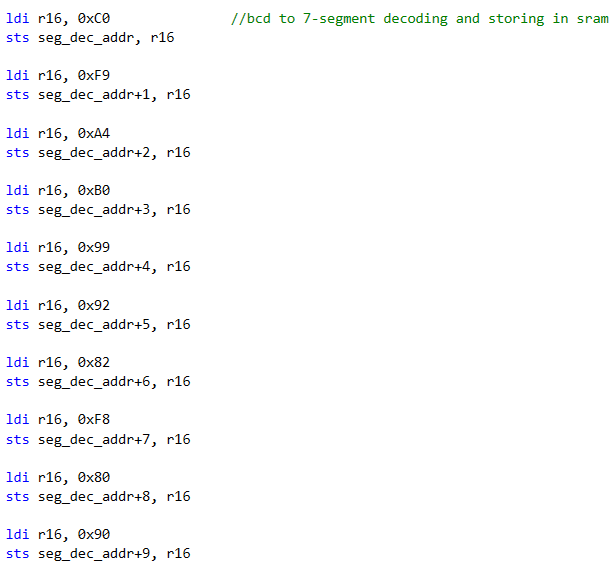
\includegraphics[width=0.8\linewidth]{./results/lab2_dec_data.png}
			\caption{Store the decoded numbers for 7-segment}
		\end{subfigure}%
		~
		\begin{subfigure}[t]{0.5\textwidth}
			\centering
			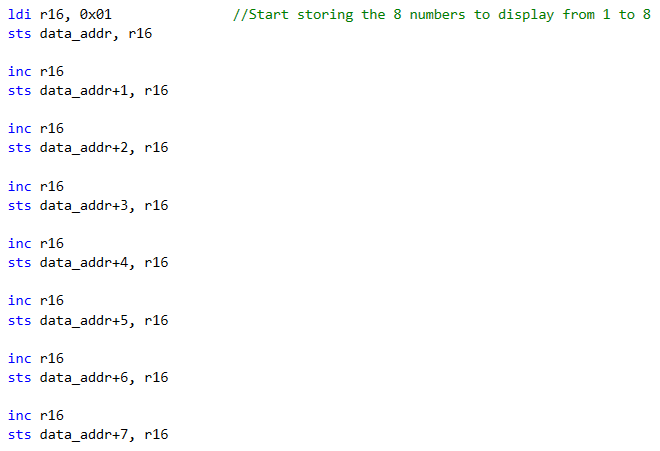
\includegraphics[width=\linewidth]{./results/lab2_display_data.png}
			\caption{Store the numbers to display}
		\end{subfigure}
	
		\begin{subfigure}[t]{0.5\textwidth}
			\centering
			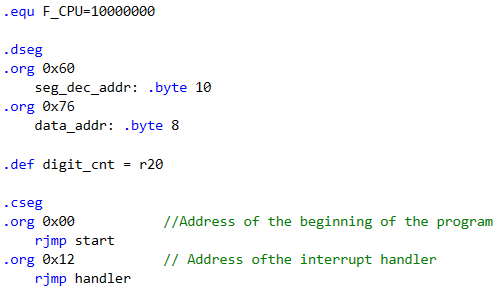
\includegraphics[width=\linewidth]{./results/lab2_malloc.png}
			\caption{Memory allocation for our data in SRAM}
		\end{subfigure}%
		~
		\begin{subfigure}[t]{0.5\textwidth}
			\centering
			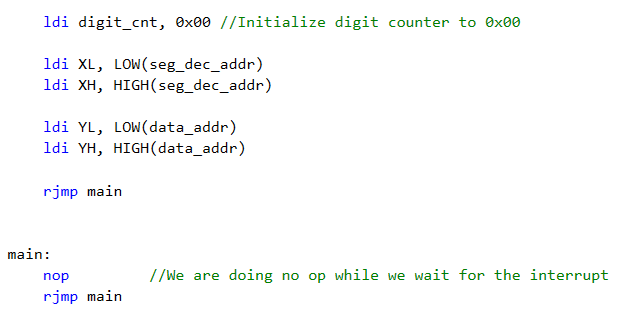
\includegraphics[width=\linewidth]{./results/lab2_init_main.png}
			\caption{Initialize X and Y register for reading data}
		\end{subfigure}	
	\end{figure}
	
	\pagebreak
	\begin{figure}[h!]
		\centering
		\begin{subfigure}[t]{0.5\textwidth}
			\centering
			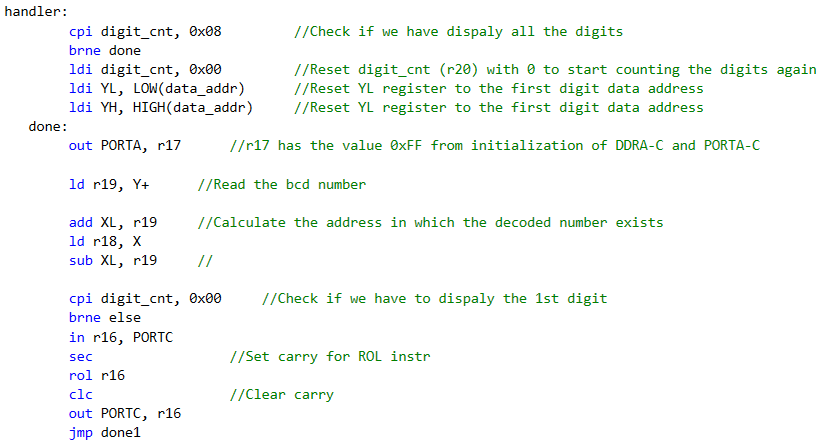
\includegraphics[width=0.9\linewidth]{./results/lab2_handler_a.png}
			\caption{Interrupt handler - part A}
		\end{subfigure}%
		~
		\begin{subfigure}[t]{0.5\textwidth}
			\centering
			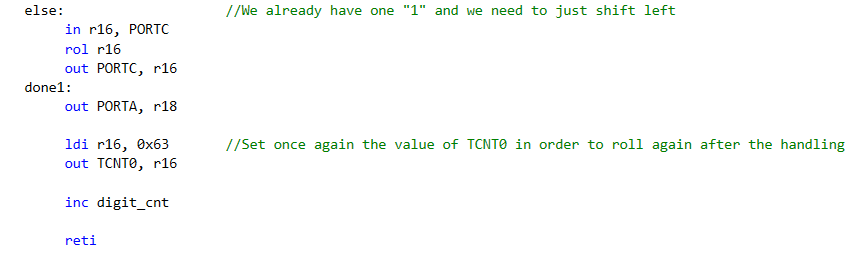
\includegraphics[width=1.2\linewidth]{./results/lab2_handler_b.png}
			\caption{Interrupt handler - part B}
		\end{subfigure}	
	\end{figure}
	
	\noindent
	\textbf{Προσομοίωση Αποτελεσμάτων} \\
	\noindent
	Όπως φαίνεται στην εικόνα 3 όλοι οι καταχωρητές DDRA, DDRC, PORTA και PORTC αρχικοποιούνται με τις σωστές τιμές, όπως περιγράφτηκε παραπάνω. Στην ίδια εικόνα βλέπουμε, επίσης, ότι οι δέκα αποκωδικοποιημένοι αριθμοί, καθώς και οι οχτώ αριθμοι από 1 εως 8 που θέλουμε να εμφανίσουμε στα 7-segments, έχουν αποθηκευτεί σωστά στην SRAM του μικροελεγκτή AVR. \\
	
	\noindent
	Παράλληλα, στις εικόνες (a) εως (h) βλέπουμε ότι κάθε φορά που έρχεται το interrupt, εκτελείται σωστά ο handler και κάθε φορά εμφανίζεται στο κατάλληλο ψηφίο η σωστή τιμή που διαβάσαμε από τη μνήμη. Επιπλέον, μια σημαντική παρατήρηση είναι ότι στο PORTC κάθε φορά υπάρχει ένας "1", δηλαδή ενεργοποιείται ένα ψηφίο τη φορά και επομένος εμφανίζουμε τον αριθμό BCD που διαβάσαμε μόνο στο ενεργοποιημένο 7-segment display. \\
	
	\noindent
	Πιο αναλυτικά, στην εικόνα (b) μετά την εκτέλεση του handler, η έξοδος PORTA έχει την τιμή 0x79 (αριθμός 1 σε BCD) και το PORTC την τιμή 0x01 (ενεργοποιημένο το πρώτο ψηφίο). Στην επόμενη εκτέλεση του handler (εικόνα (c)), η θύρα A, αλλάζει σε 0xΑ4 (αριθμός 2 σε BCD) και τo "1" έχει ολισθήσει στο δεύτερο ψηφίο. Η ίδια διαδικασία επαναλαμβάνεται μέχρι και τον 8ο αριθμό που διβάζουμε από τη μνήμη και ξανά από την αρχή. Αυτό έχει ως αποτέλεσμα τελικά να παρατηρούμε στα οχτώ 7-segment LED τους αριθμούς 1 έως 8 οι οποίοι αποθηκεύτηκαν στη μνήμη.
	
	\begin{figure}[h!]
		\centering
		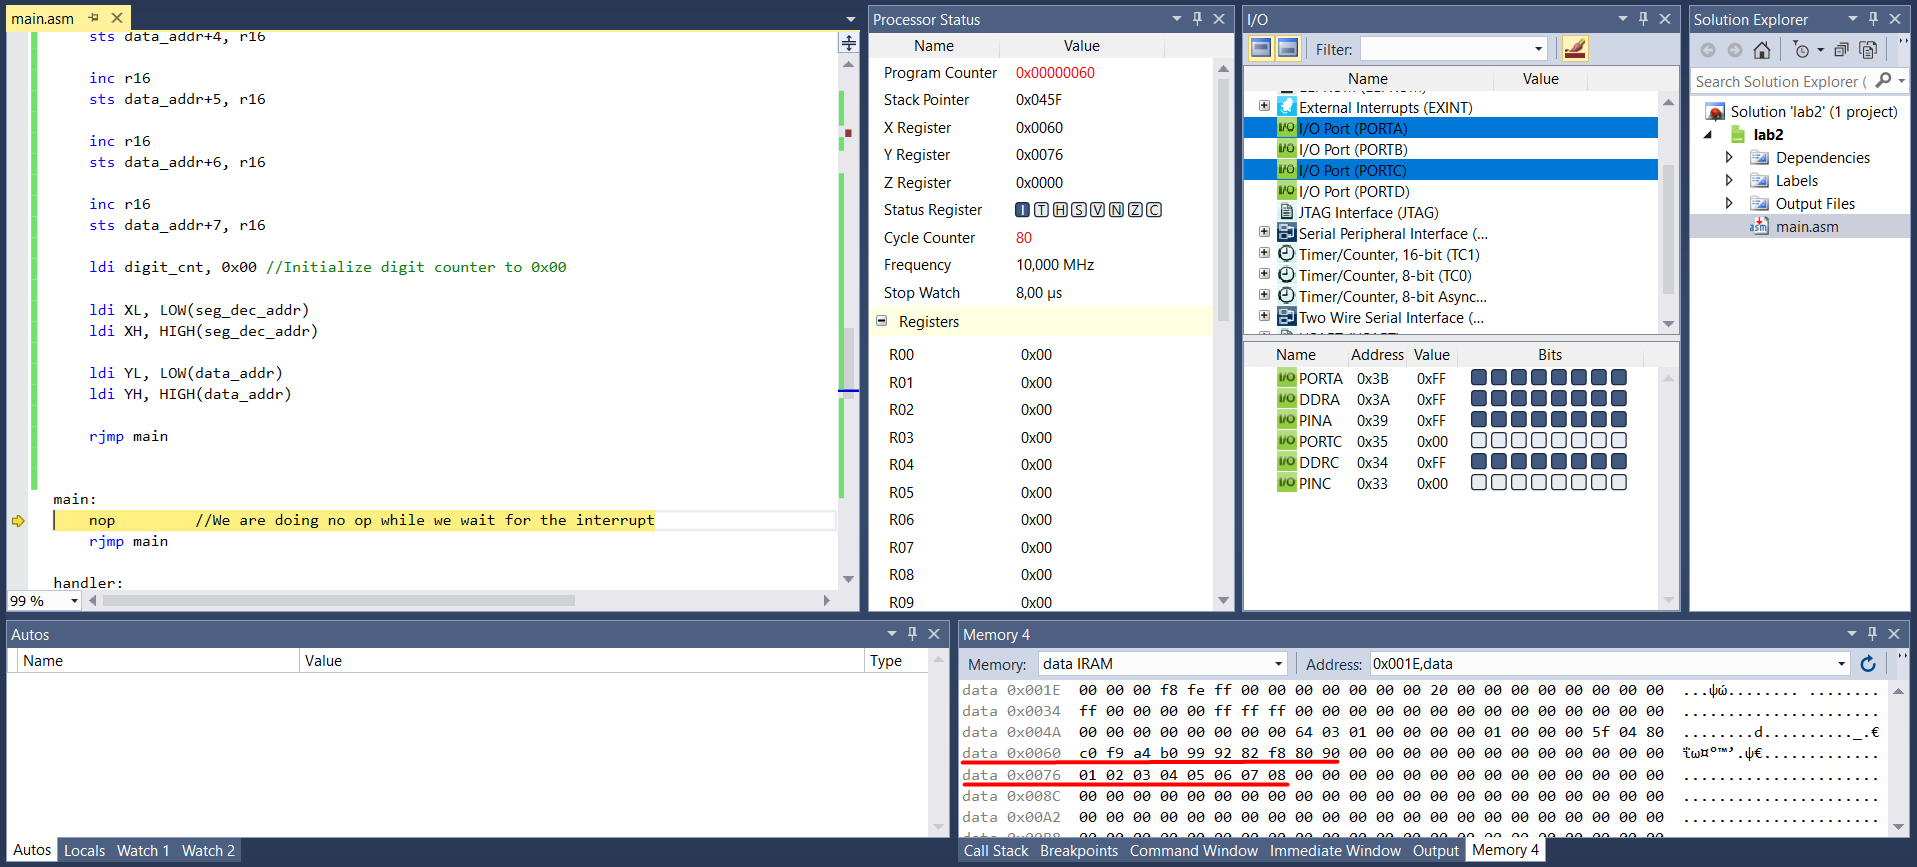
\includegraphics[width=\linewidth]{./results/lab2_after_init.png}
		\caption{Results from Αtmel Studio 7 - Ιnitialization of register and memory}
	\end{figure}
	
	\pagebreak
	\begin{figure}[h!]
		\centering
		\begin{subfigure}[t]{0.5\textwidth}
			\centering
			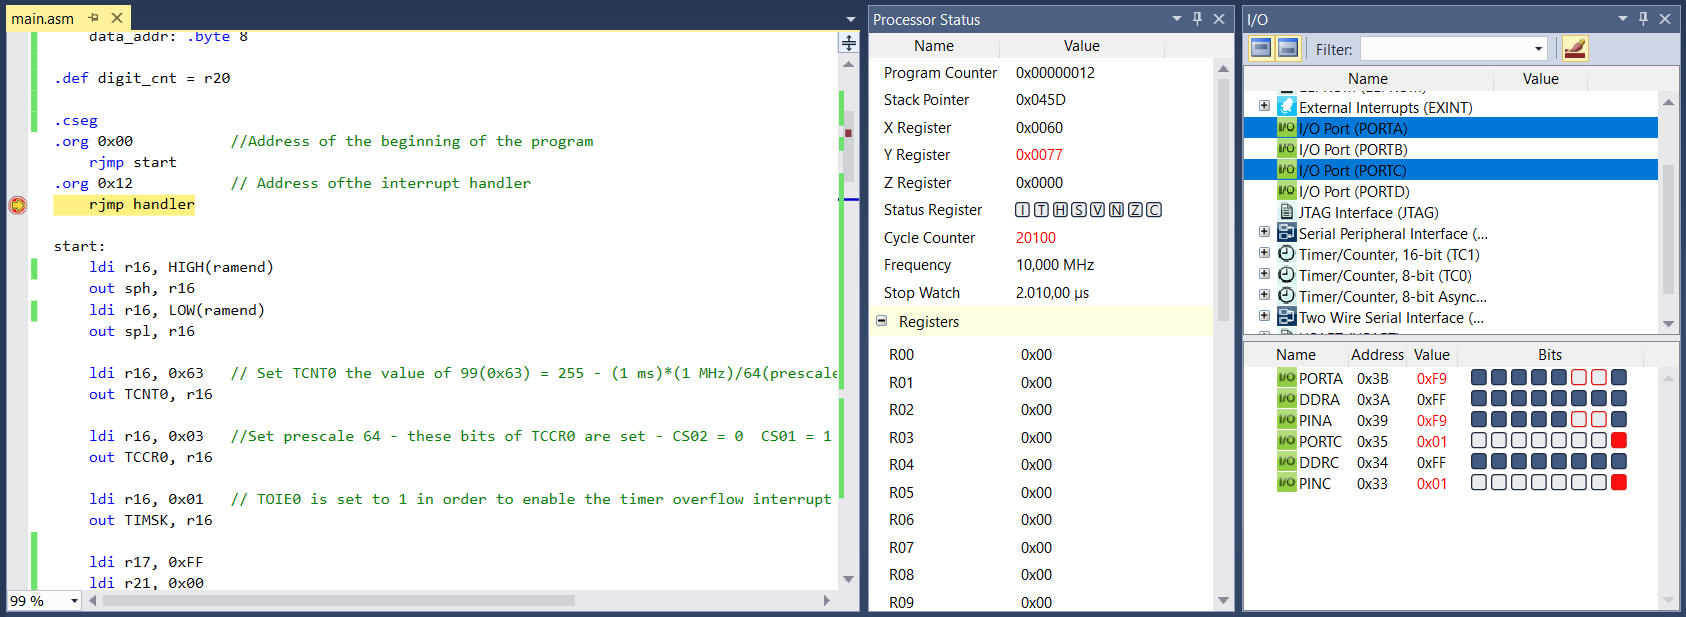
\includegraphics[width=\linewidth]{./results/lab2_sim_dig1.png}
			\caption{Results from Αtmel Studio 7 - Display digit 1}
		\end{subfigure}%
		~
		\begin{subfigure}[t]{0.5\textwidth}
			\centering
			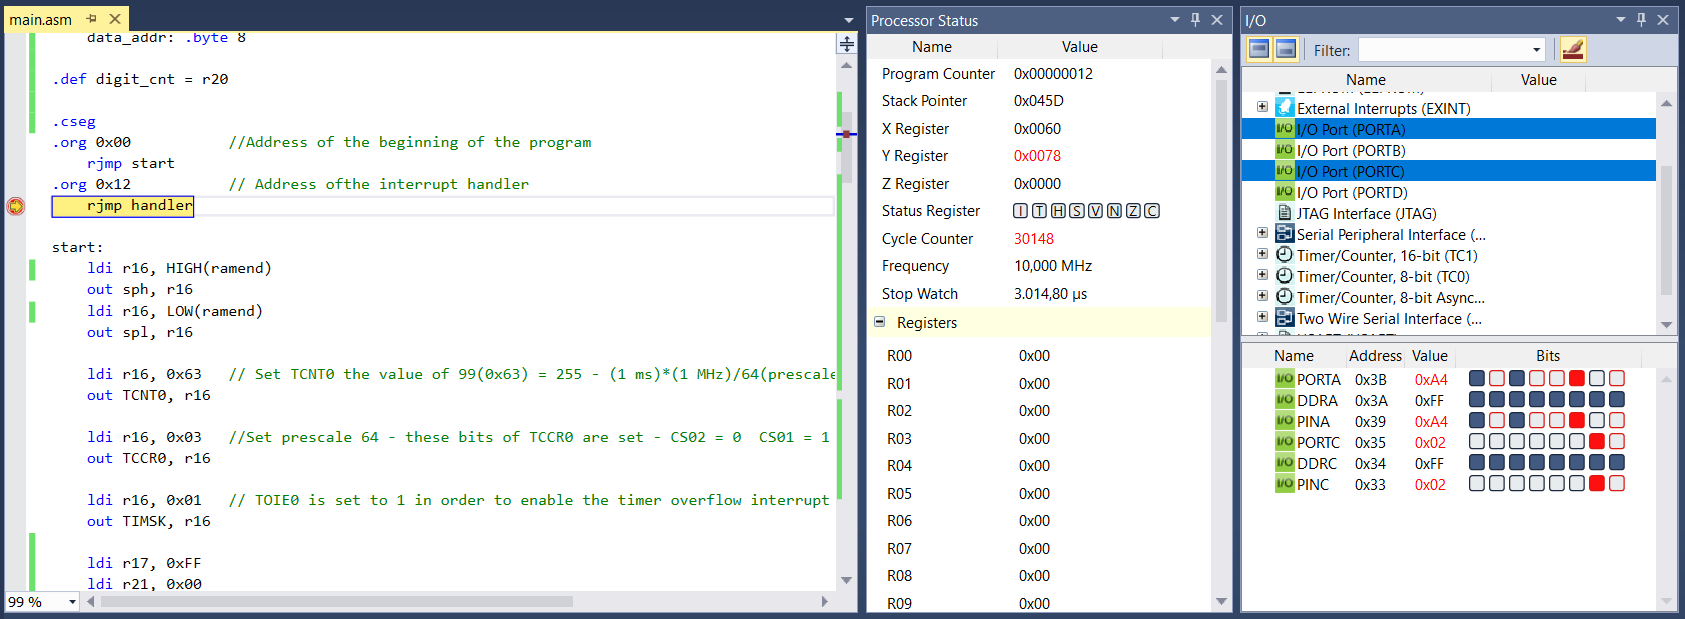
\includegraphics[width=\linewidth]{./results/lab2_sim_dig2.png}
			\caption{Results from Αtmel Studio 7 - Display digit 2}
		\end{subfigure}%
		
		\begin{subfigure}[t]{0.5\textwidth}
			\centering
			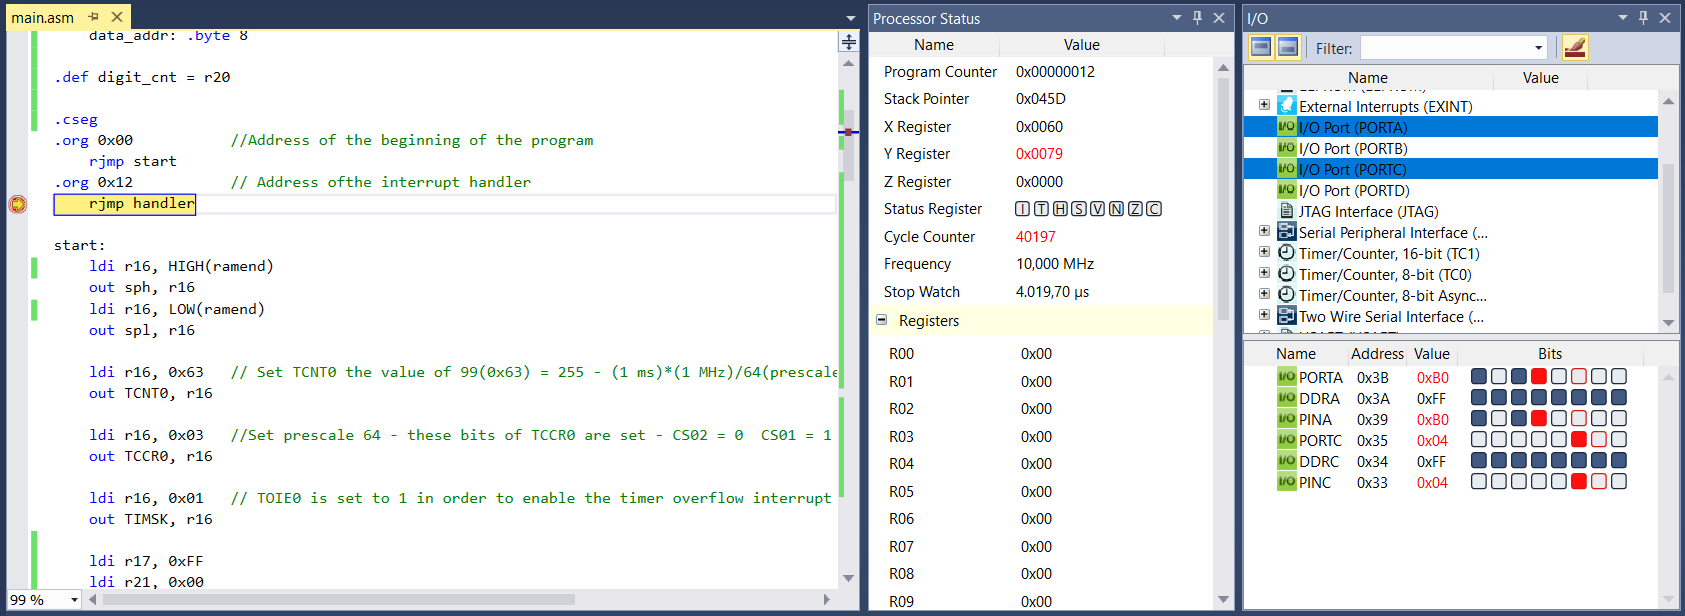
\includegraphics[width=\linewidth]{./results/lab2_sim_dig3.png}
			\caption{Results from Αtmel Studio 7 - Display digit 3}
		\end{subfigure}%
		~
		\begin{subfigure}[t]{0.5\textwidth}
			\centering
			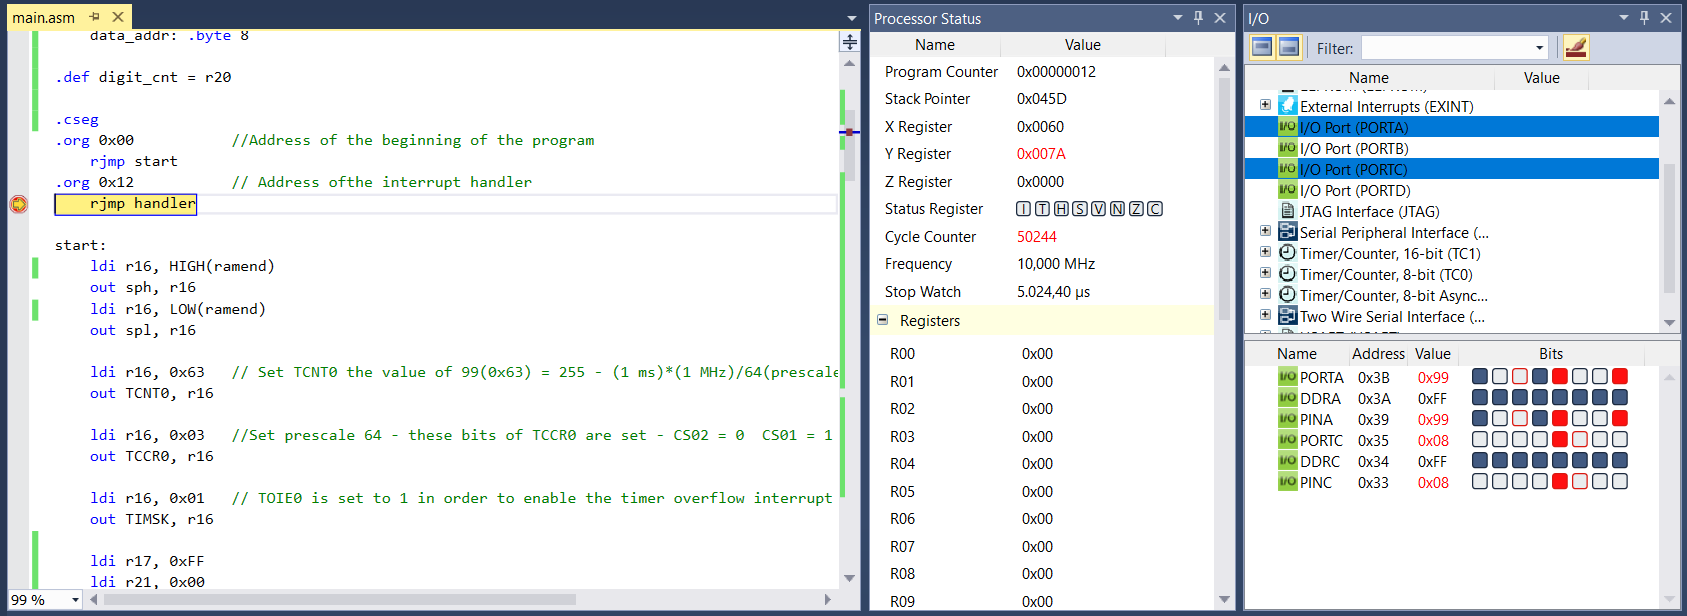
\includegraphics[width=\linewidth]{./results/lab2_sim_dig4.png}
			\caption{Results from Αtmel Studio 7 - Display digit 4}
		\end{subfigure}%
	
		\begin{subfigure}[t]{0.5\textwidth}
			\centering
			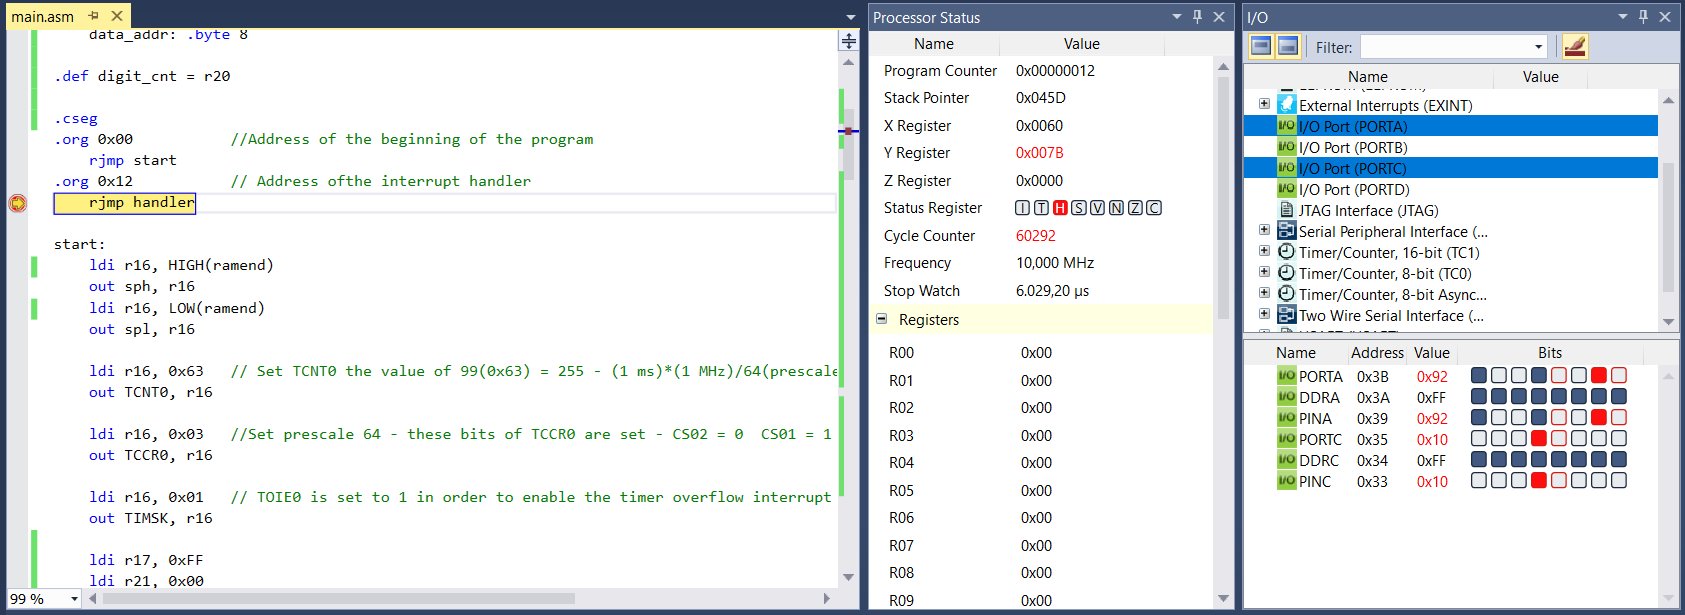
\includegraphics[width=\linewidth]{./results/lab2_sim_dig5.png}
			\caption{Results from Αtmel Studio 7 - Display digit 5}
		\end{subfigure}%
		~
		\begin{subfigure}[t]{0.5\textwidth}
			\centering
			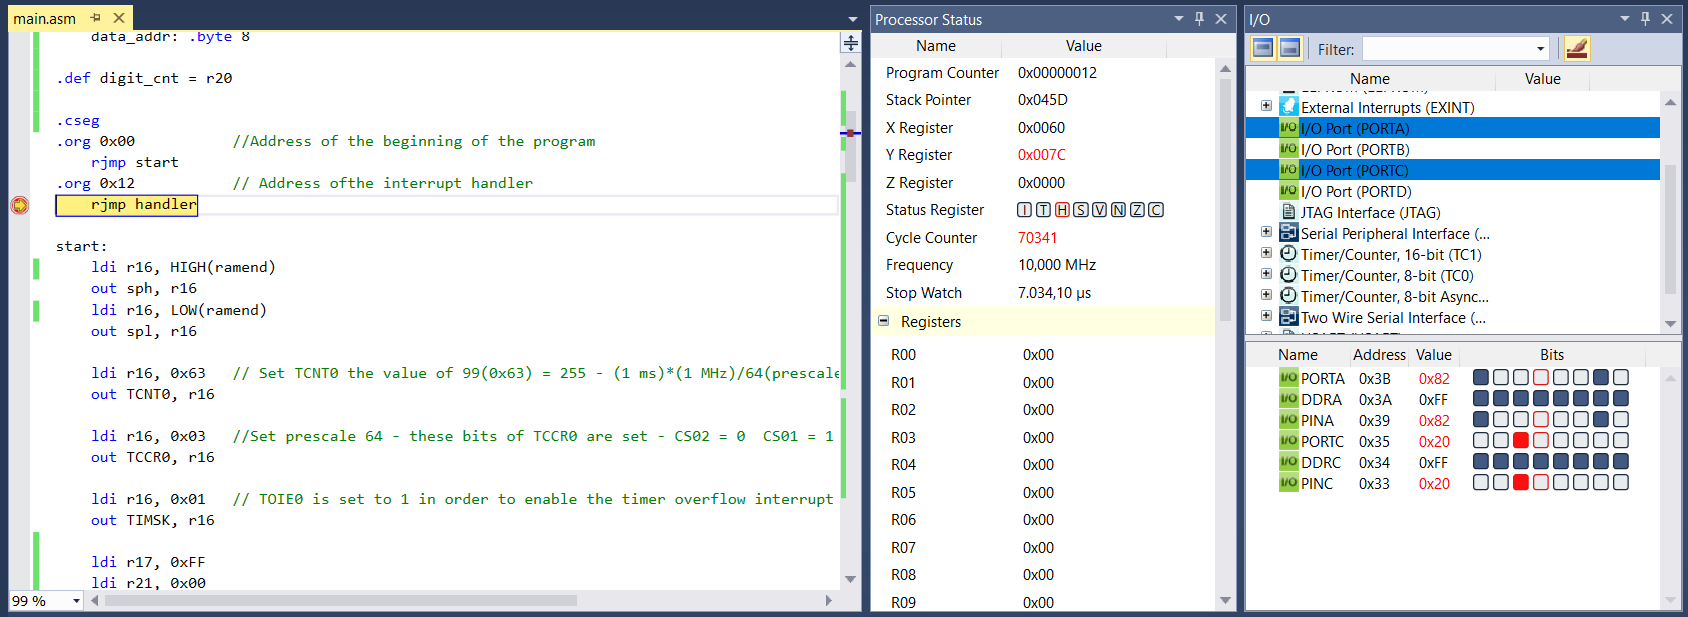
\includegraphics[width=\linewidth]{./results/lab2_sim_dig6.png}
			\caption{Results from Αtmel Studio 7 - Display digit 6}
		\end{subfigure}%
		
		\begin{subfigure}[t]{0.5\textwidth}
			\centering
			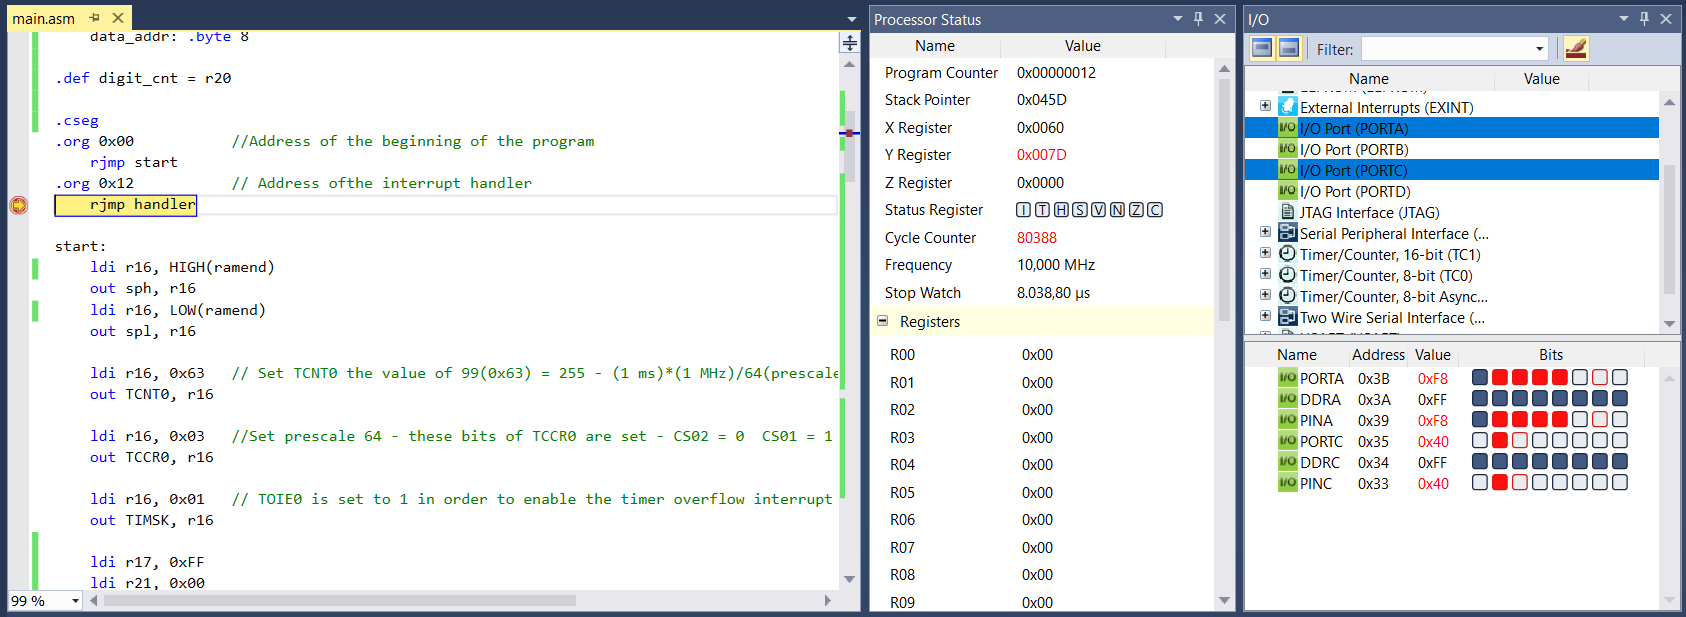
\includegraphics[width=\linewidth]{./results/lab2_sim_dig7.png}
			\caption{Results from Αtmel Studio 7 - Display digit 7}
		\end{subfigure}%
		~
		\begin{subfigure}[t]{0.5\textwidth}
			\centering
			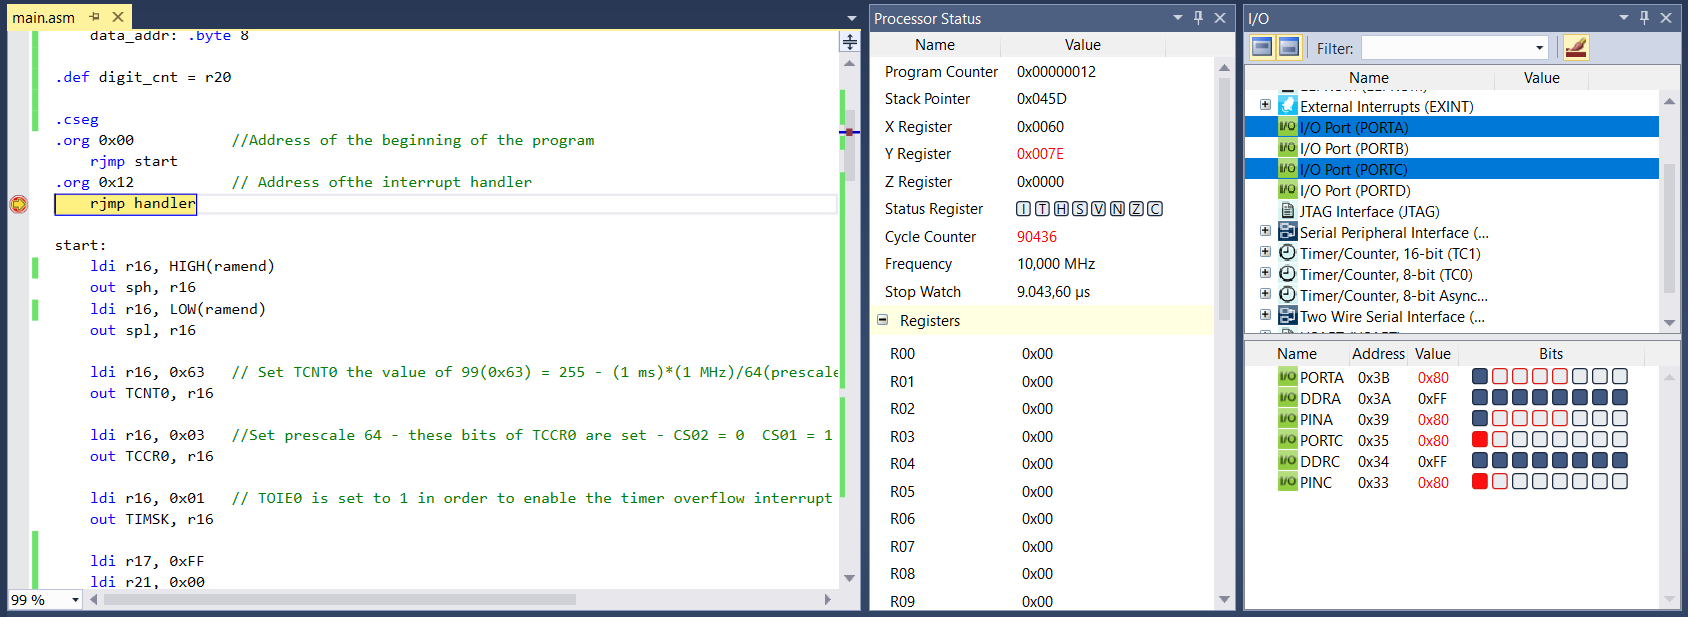
\includegraphics[width=\linewidth]{./results/lab2_sim_dig8.png}
			\caption{Results from Αtmel Studio 7 - Display digit 8}
		\end{subfigure}
	
	\end{figure}


\end{document}
